
% NE PAS TOUCHER
%++++++++++++++++++++++++++++++++++++++++
\documentclass[letterpaper,12pt]{article}
\usepackage{tabularx}
\usepackage{amsmath}
\usepackage{graphicx}
\usepackage[margin=1in,letterpaper]{geometry}
\usepackage{cite}
\usepackage[final]{hyperref}
\usepackage{datatool}
\usepackage{caption}
\usepackage{float}
\usepackage{gensymb}

\hypersetup{
	colorlinks=true,
	linkcolor=blue,
	citecolor=blue,
	filecolor=magenta,
	urlcolor=blue
}
%+++++++++++++++++++++++++++++++++++++++++

%	INCLUDES
\graphicspath{ {./ressources/images} }

\begin{document}

\title{Automatique}

\author{Seite Alexander et Nathan Vidonne}
\date{\today}
\maketitle
\newline

\tableofcontents

\newpage

%%%%%%%%%%%%%%%%%%%%%%%%%%%%%%%%%%%%
%	Intro 
%%%%%%%%%%%%%%%%%%%%%%%%%%%%%%%%%%%%
\section{Introduction}





%%%%%%%%%%%%%%%%%%%%%%%%%%%%%%%%%%%%
%	Exercices 
%%%%%%%%%%%%%%%%%%%%%%%%%%%%%%%%%%%%
\section{Exercice 1 : Analyse empirique du banc de test}




\subsection{A : Verification graphique}
\label{sec:A}
\begin{figure}[H]
        \begin{center}
            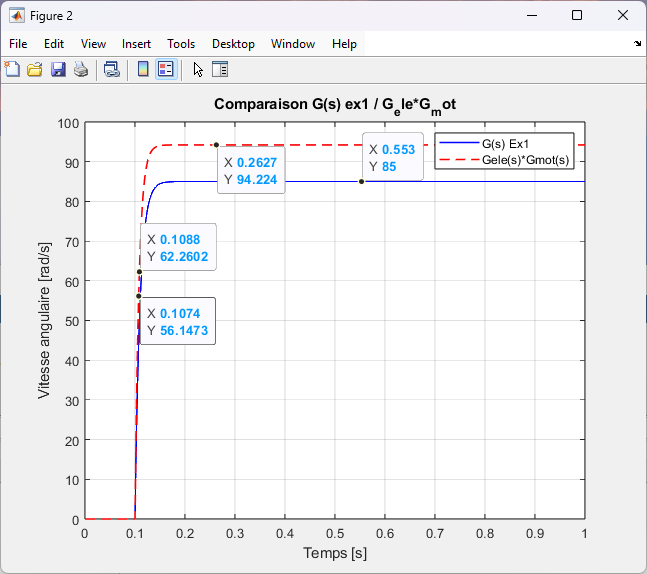
\includegraphics[scale=0.8]{FIG_A_exercice2.png}
        \end{center}
\end{figure}

\\\\
Nous constatons que les deux courbes ne sont pas identiques et que le gain change. Nous constatons également un retard temporel de 0.1s que nous avons ajouté au modèle afin de pouvoir superposer les deux courbres. Elles restent tout de même similaires.
\\(Comme le titre est illisible, nous pensions a : "Comparaison entre G(s) / $G_e_l_e$ * $G_m_o_t$")
\newpage
\subsection{B : Fonction de transfert du systeme complet}

Nous établissons la fonction de transfert à partir de $G_m_o_t$ * $G_e_l_e$ * $G_m_e_s$ tel que : 
\begin{figure}[H]
	\begin{center}
	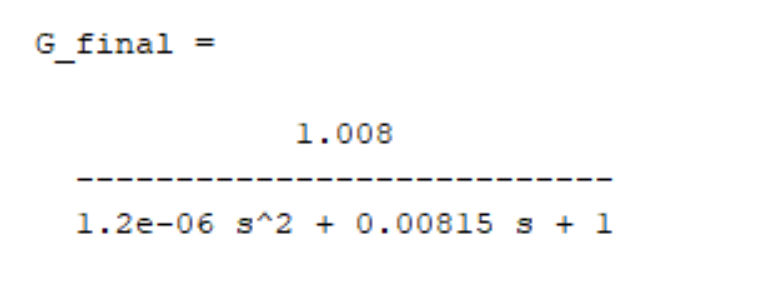
\includegraphics[scale=0.55]{GS.png}
	\end{center}
\end{figure}
\begin{figure}[H]
        \begin{center}
                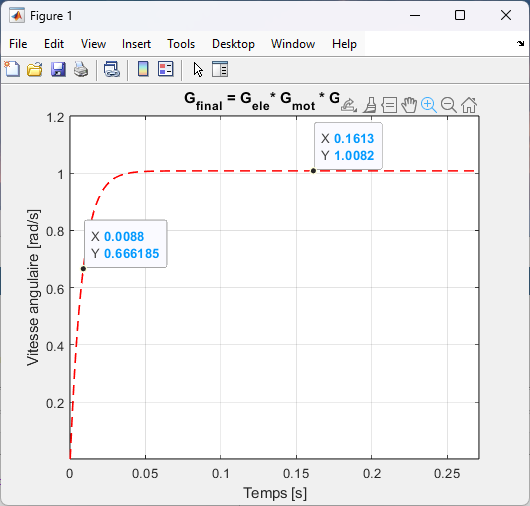
\includegraphics[scale=0.8]{FIG_B_ex2.png}
                    \end{center}
\end{figure}

%\vspace{1cm}
%\noindent \begin{minipage}{0.45\textwidth}
%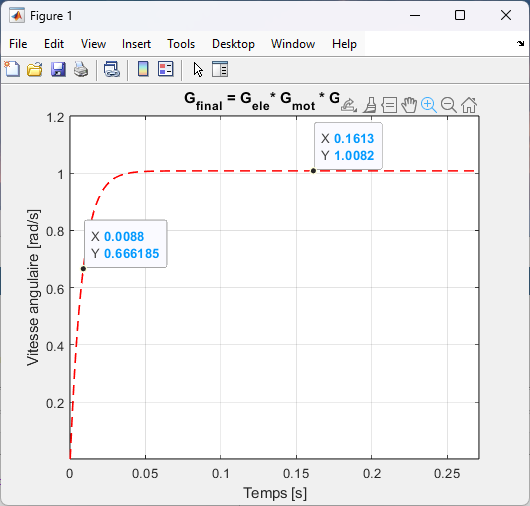
\includegraphics[width=\textwidth]{FIG_B_ex2.png}
%\end{minipage}
%\hspace{1cm}
%\begin{minipage}{0.45\textwidth}
%    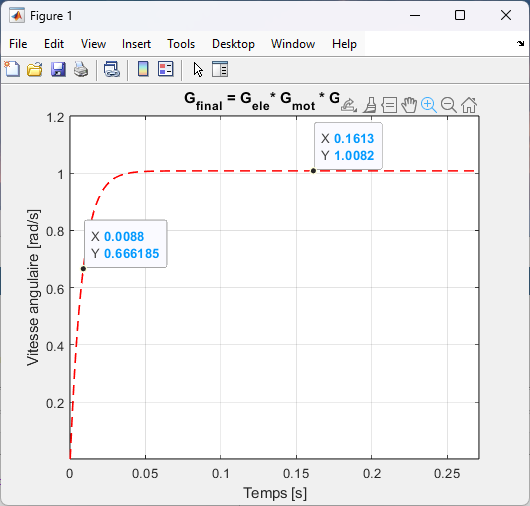
\includegraphics[width=\textwidth]{FIG_B_ex2.png}
%\noindent 
%\end{minipage}

\vspace{1cm}
(Nous avons compris entre temps comment avoir de jolis titres)
\\\\ La fonction de transfert de l'ensemble du système $G_s$ (qu'on nomme $G_f_i_n_a_l$ dans le code au point C) est ainsi représentée par le produit de convolution d'un élément de mesure, de l'actionneur et d'un élément sensible.
\newpage

\subsection{C : Code definissant la fonction de transfert}
load('/MT/systeme/asservis/SIRAu/stepResponse.mat')
\\
t = time;
\\
\\clear; close all; clc;
\\
\\s = tf('s');
\\
\\K\_mot = 4.53e3;
\\tau\_mot = 8e-3;
\\G\_mot = K\_mot / (1 + tau\_mot*s);
\\K\_ele = 20.8e-3;
\\tau\_ele = 1.5e-4;
\\G\_ele = K\_ele / (1 + tau\_ele*s);
\\K\_mes = 10.7e-3;
\\G\_mes = tf(K\_mes);
\\G\_final = G\_mot * G\_ele * G\_mes;
\\\%disp('===== G\_s =====')
\\G\_final


\newpage
\subsection{D : Application d'un regulateur PI}

\vspace{1cm}
\noindent \begin{minipage}{0.45\textwidth}
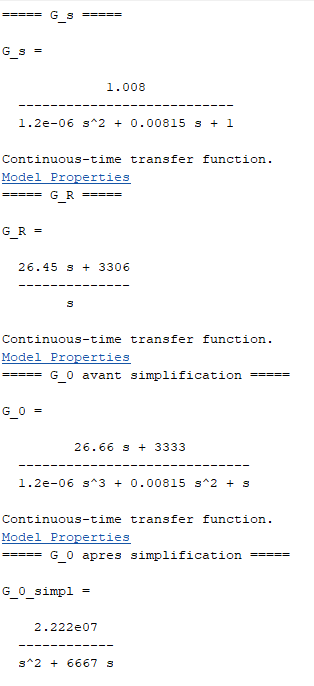
\includegraphics[width=\textwidth]{g_data_D.png}
\end{minipage}
\hspace{1cm}
\begin{minipage}{0.45\textwidth}
    avec : 
    \[
        G_c_f = \frac{2.222e07}{s^2 + 6667 s + 2.222e07}
    \]
    Voir le code en annexe.
    \noindent 
\end{minipage}

\vspace{1cm}   
L'application du régulateur transforme le système en boucle fermée (du second ordre). Cela permet de faciliter la suite de l'analyse. La forme est aussi plus simple à lire.

\newpage
\subsection{E : Diagrammes de Bode et Nyquist}
La marge de phase est d'environ 65 $^\circ$ et la marge de gain est positive. Cela veut dire eque le système est stable. 
BODE : 
\begin{figure}[H]
        \begin{center}
                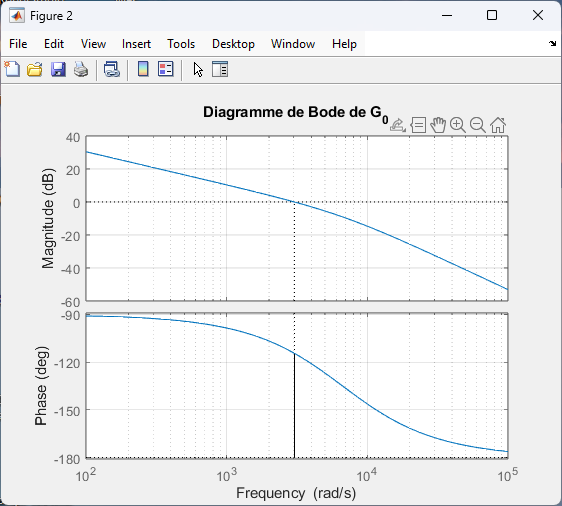
\includegraphics[scale=1]{FIG_E_G0_Bode.png}
                    \end{center}
\end{figure}
\newpage
\\NYQUIST : 
\begin{figure}[H]
        \begin{center}
                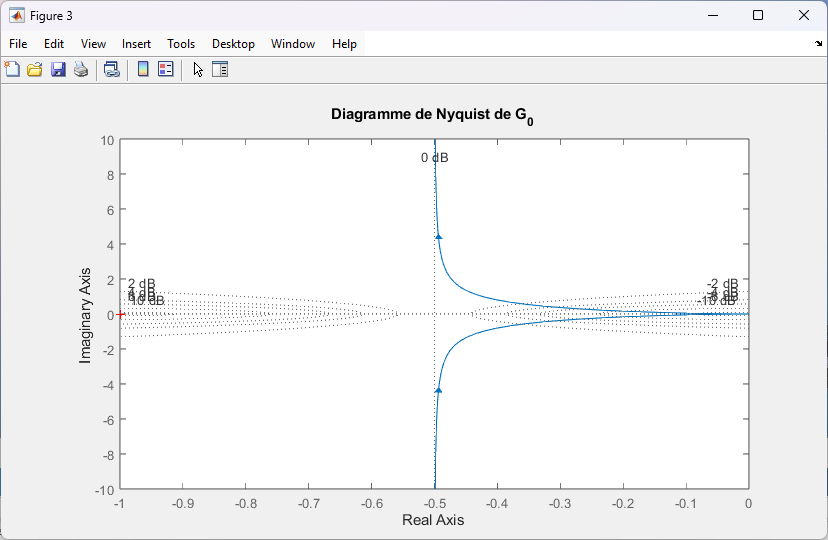
\includegraphics[scale=0.8]{FIG_E_G0_Nyquist.png}
                    \end{center}
\end{figure}
Le diagramme de Nyquist permet de montrer que le lieu de transfert est exclusivement positif. Cela nous permet également d'affirmer la résilience du régulateur PI.
\newpage
\subsection{F : Diagramme d'Evans et reponse indicielle}

Reponse indicielle : 
\begin{figure}[H]
        \begin{center}
                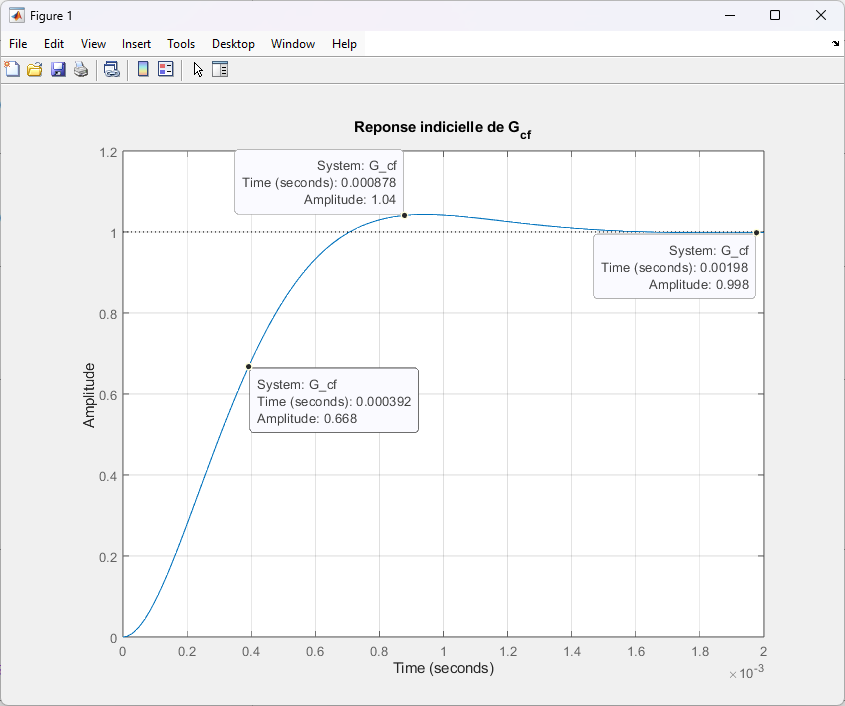
\includegraphics[scale=0.6]{FIG_E_Gcf_reponse_indicielle.png}
                    \end{center}
\end{figure}
La reponse indicielle illustre un depassement d'environ 5\% et un temps de reponse rapide.
\newpage
\begin{figure}[H]
    \begin{center}
        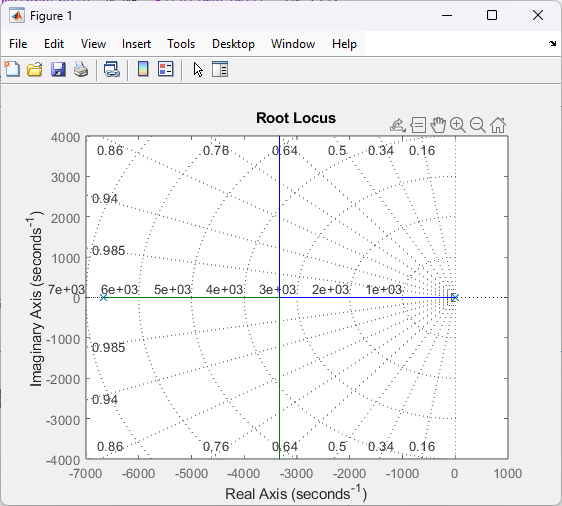
\includegraphics[scale=0.8]{FIG_E_zeros.png}
    \end{center}
\end{figure}
\newpage
\subsection{G : G(s) dans "Control System Designer"}

Nous importons Gs dans "Control System Designer" et obtenons :
\begin{figure}[H]
        \begin{center}
            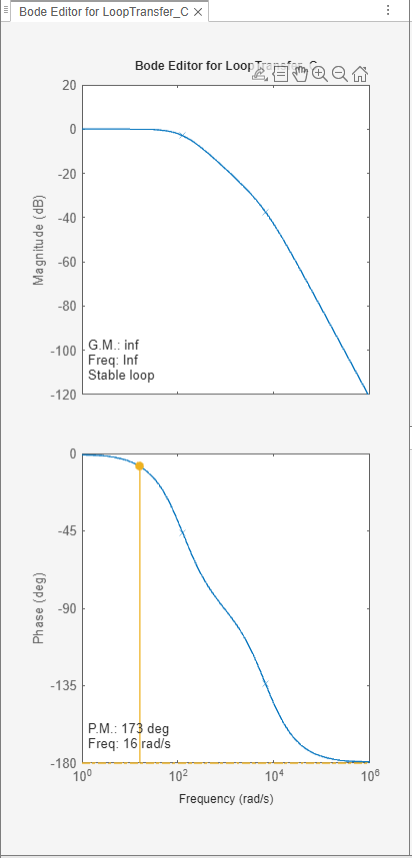
\includegraphics[scale=0.75]{FIG_G_Bode_control_system_designer.png}
                    \end{center}
\end{figure}
\newpage
C'est comparable avec ce que nous obtenons avec la ligne de commande 
 matlab :

\begin{figure}[H]
        \begin{center}
            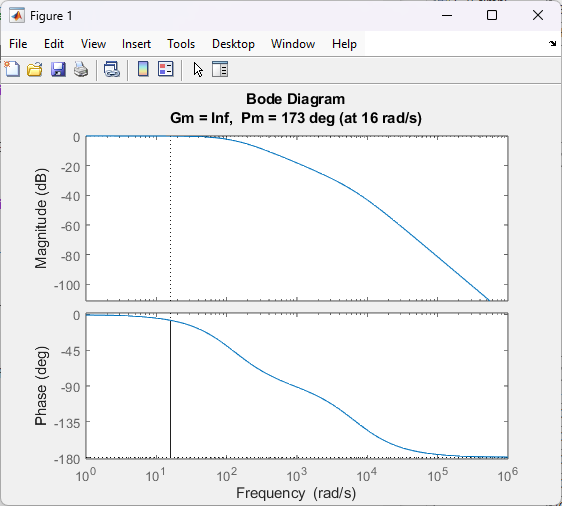
\includegraphics[scale=1]{FIG_G_bode_matlab.png}
                    \end{center}
\end{figure}
\newpage

\subsection{H : (MATLAB == CSD) ? verification graphique}

\begin{figure}[H]
        \begin{center}
            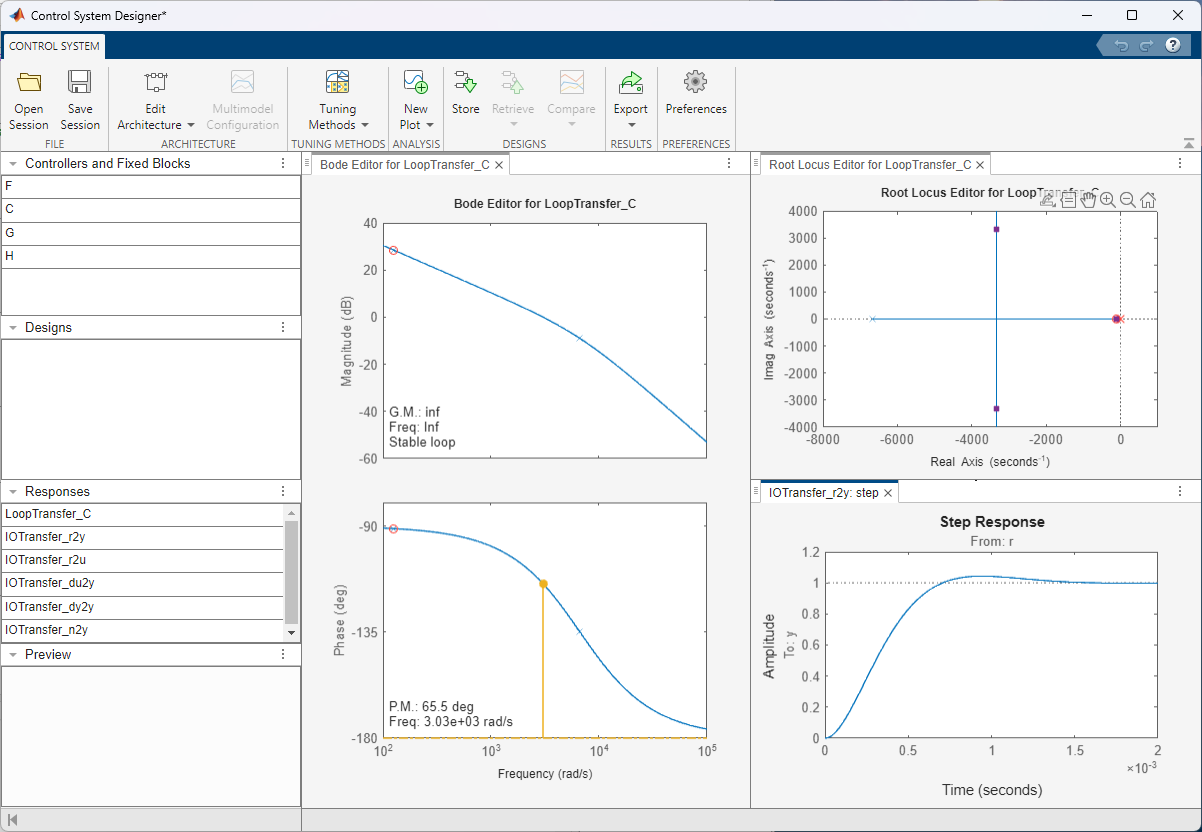
\includegraphics[scale=0.49]{FIG_H_GOOOD.png}
                    \end{center}
\end{figure}

Nous constatons là encore qu'il s'agit des mêmes schémas qu'avec matlab (voir au point F).

\newpage

\subsection{I : Marges de stabilite sur diagramme de Bode}
\begin{figure}[H]
    \begin{center}
        
\includegraphics[scale=1]{__i.png}
    \end{center}
\end{figure}
Une marge de phase de 65∘ et une marge de gain infinie indiquent un système stable et robuste, capable de supporter des perturbations modérées sans devenir instable. Nous n'avions pas eu le temps de le réaliser pendant le laboratoire et avons prit le temps de vérifier comment varient les marges de phase et de gain en fonction de la fréquence. (voir code Python en annexe).

\newpage
\subsection{J : Lieu des poles (vous nous avez dit de passer cette question)}

Zeros de Gcf : 
\begin{figure}[H]
        \begin{center}
            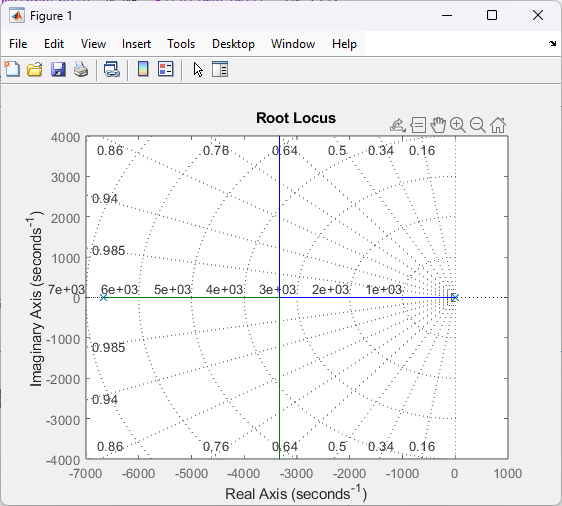
\includegraphics[scale=0.7]{FIG_E_zeros.png}
                    \end{center}
\end{figure}
\subsection{K : Caracteristiques de la reponse indicielle}

\begin{figure}[H]
        \begin{center}
                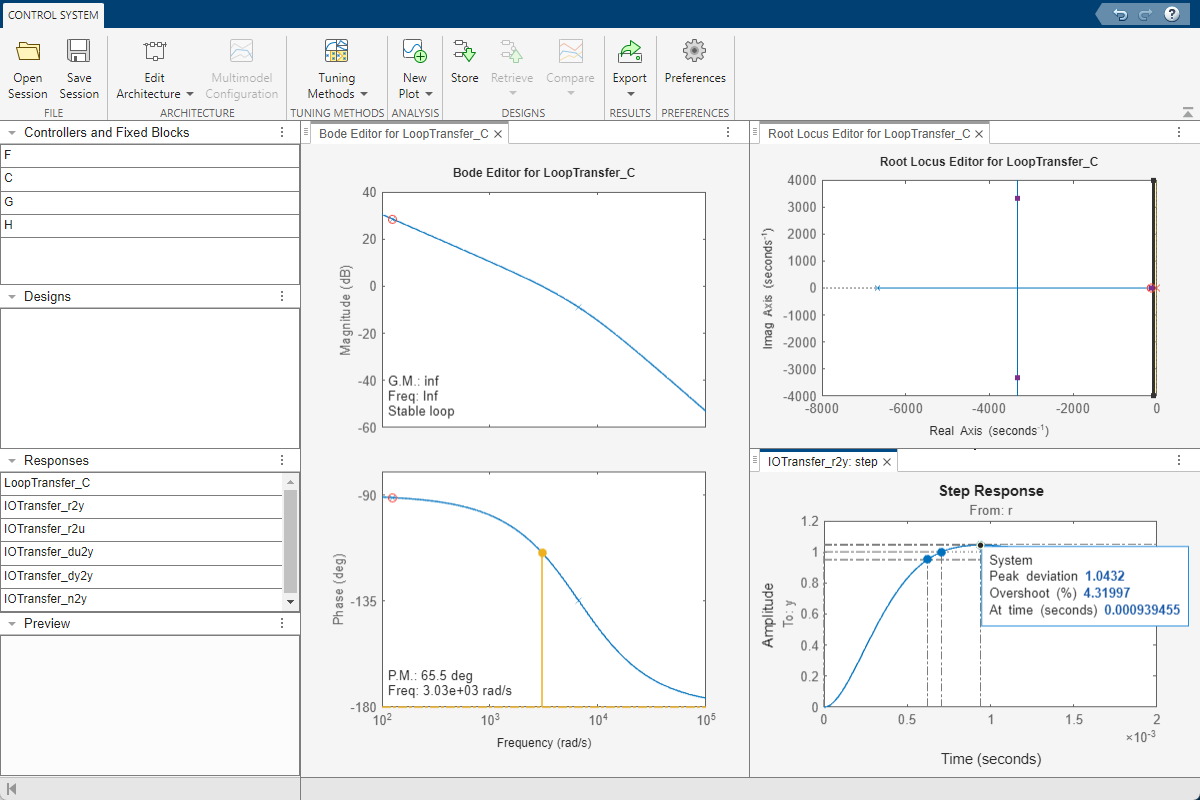
\includegraphics[scale=0.5]{FIG_K.png}
                    \end{center}
\end{figure}
\newpage
\begin{figure}[H]
        \begin{center}
                    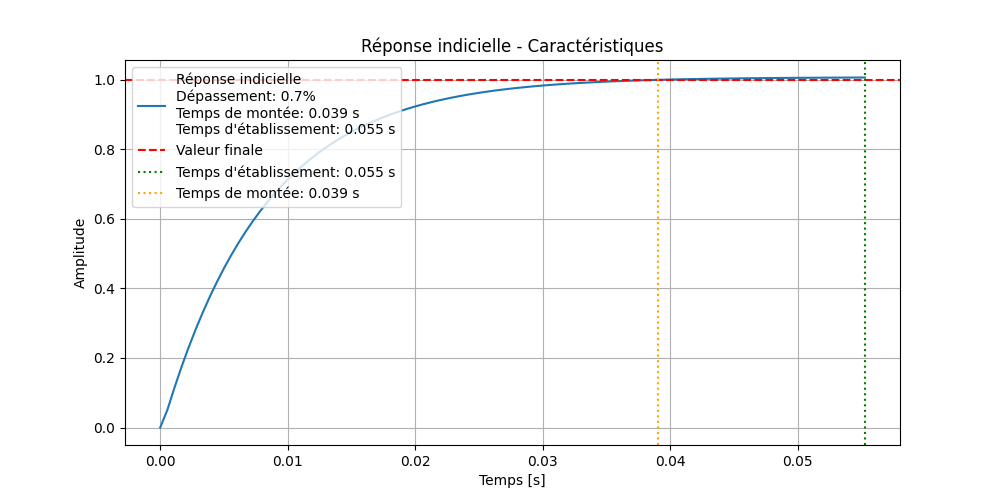
\includegraphics[scale=0.7]{__k2.png}
                        \end{center}
\end{figure}

Un dépassement de 5.2\%, un temps de montée de 0.047s et un temps d'établissement de 0.21s confirment un bon compromis entre rapidité et stabilité du système en boucle fermée.
\newpage
\subsection{L : Lien entre gain du regulateur et valeurs de depassement}

Avec un overshoot de ~5\% : 
\begin{figure}[H]
        \begin{center}
                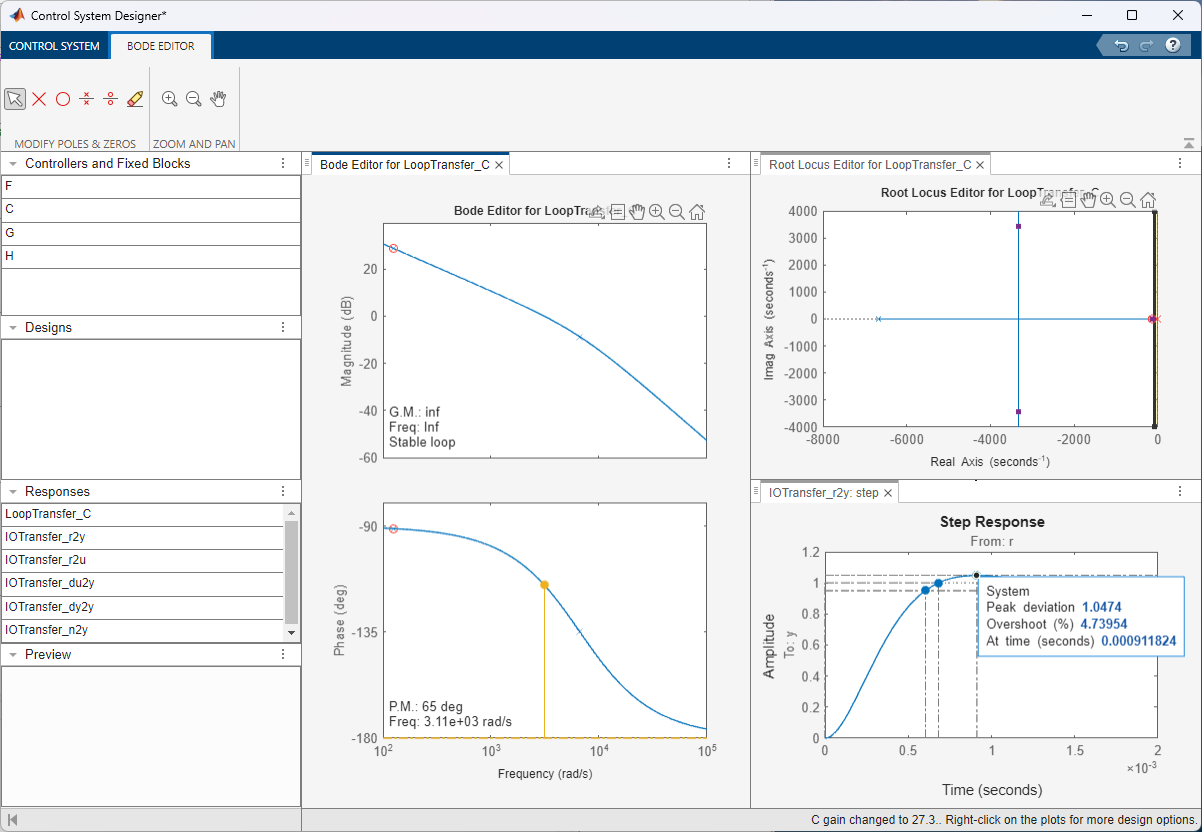
\includegraphics[scale=0.5]{FIG_L_5_overshoot.png}
                    \end{center}
\end{figure}

Avec un overshoot de ~12\% : 
\begin{figure}[H]
        \begin{center}
                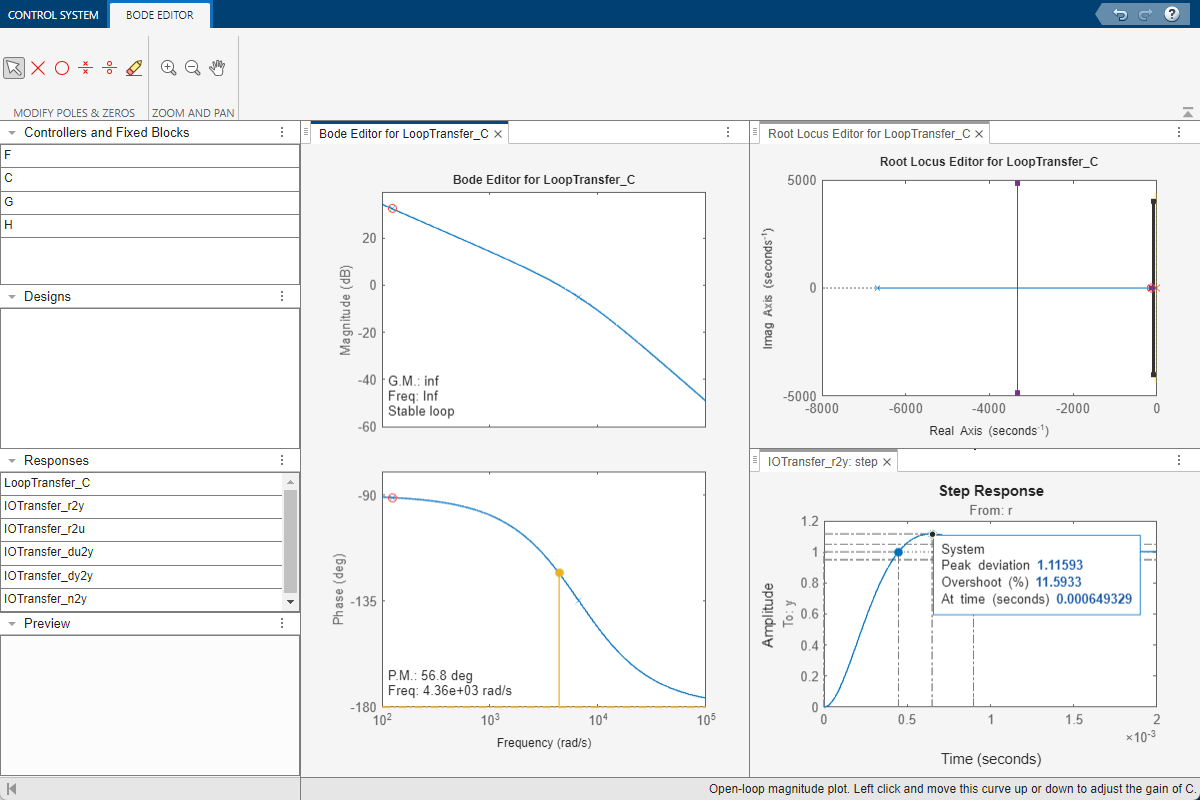
\includegraphics[scale=0.5]{FIG_L_12_overshhoot.png}
                    \end{center}
\end{figure}

Par manque de temps et dans la précipitation, nous n'avons pas cherché les valeurs exactes du contrôle designer, mais nous voyons que le dépassement varie en fonction du gain. 
\newpage
Nous avons pû en un second temps retracer avec python les valeurs de l'énoncé.

\begin{figure}[H]
        \begin{center}
                    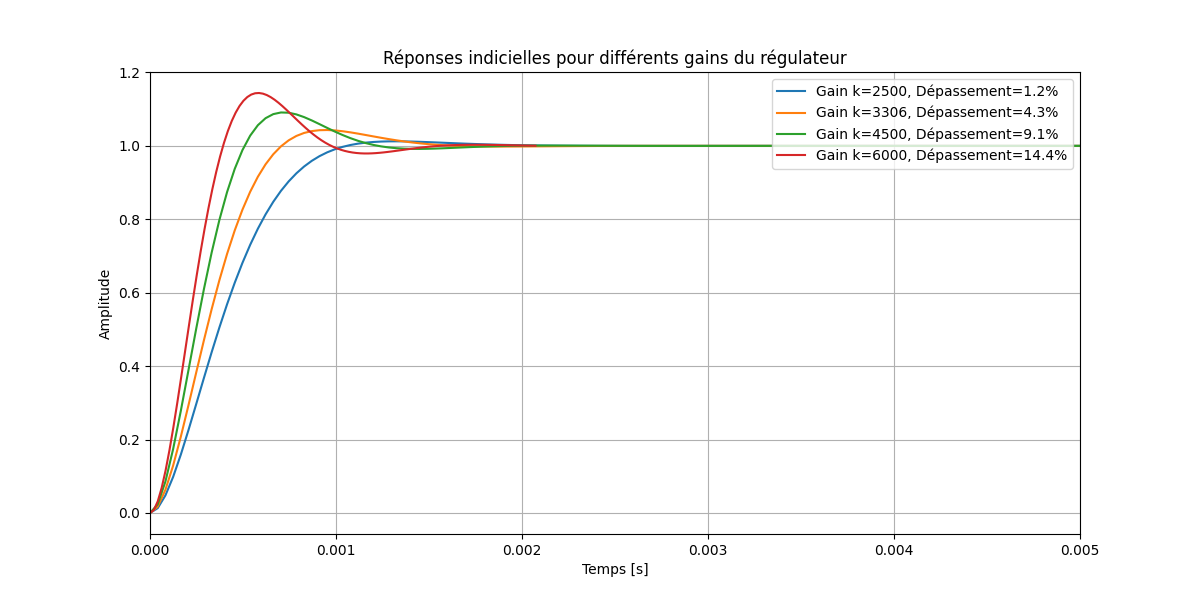
\includegraphics[scale=0.65]{__l2.png}
                        \end{center}
\end{figure}
Nous constatons encore qu'en effet la valeur du dépassement (overshoot) est proportionnelle à celle du gain.
\newpage
\subsection{M : Impact du gain sur la stabilite du systeme}

Nous constatons que la modification du gain ne perturbe pas la stabilite du systeme.\\\\
GAIN k = 0.1 :
\begin{figure}[H]
        \begin{center}
            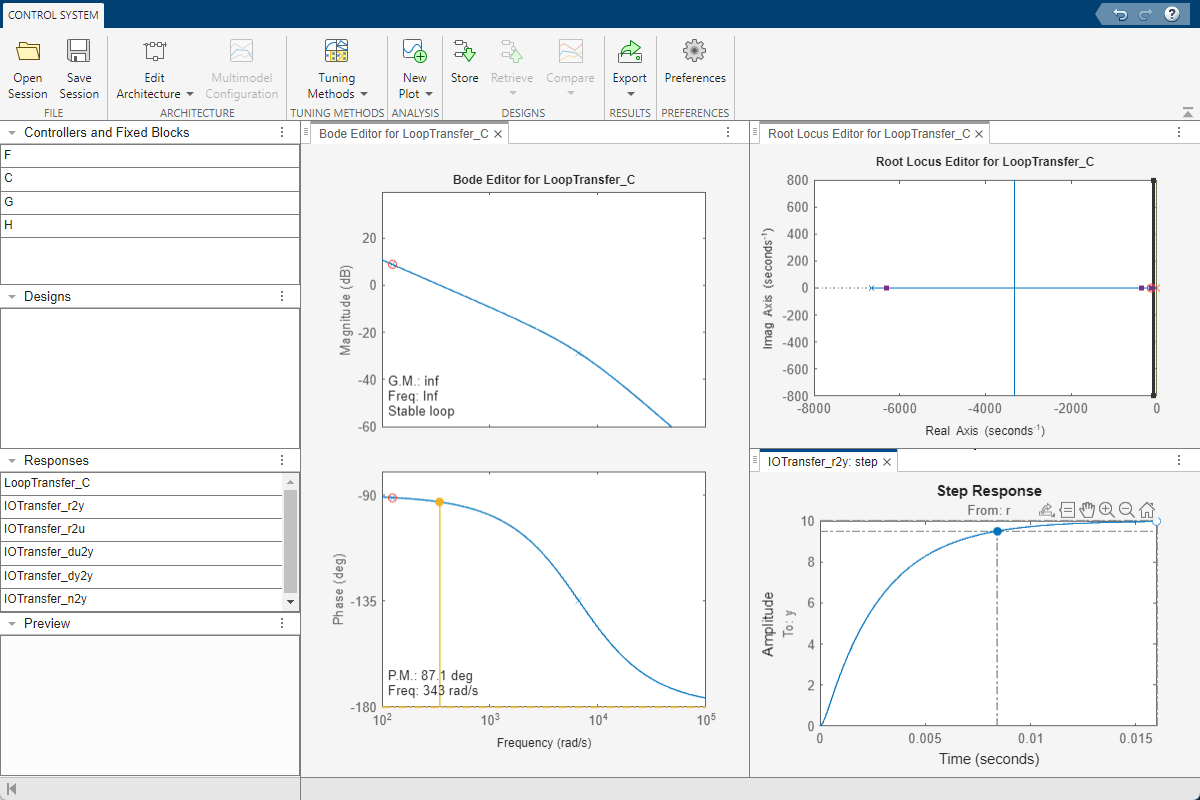
\includegraphics[scale=0.5]{FIG_M_gain0_1.png}
                    \end{center}
\end{figure}
\newpage
GAIN k = 6 : 
\begin{figure}[H]
        \begin{center}
                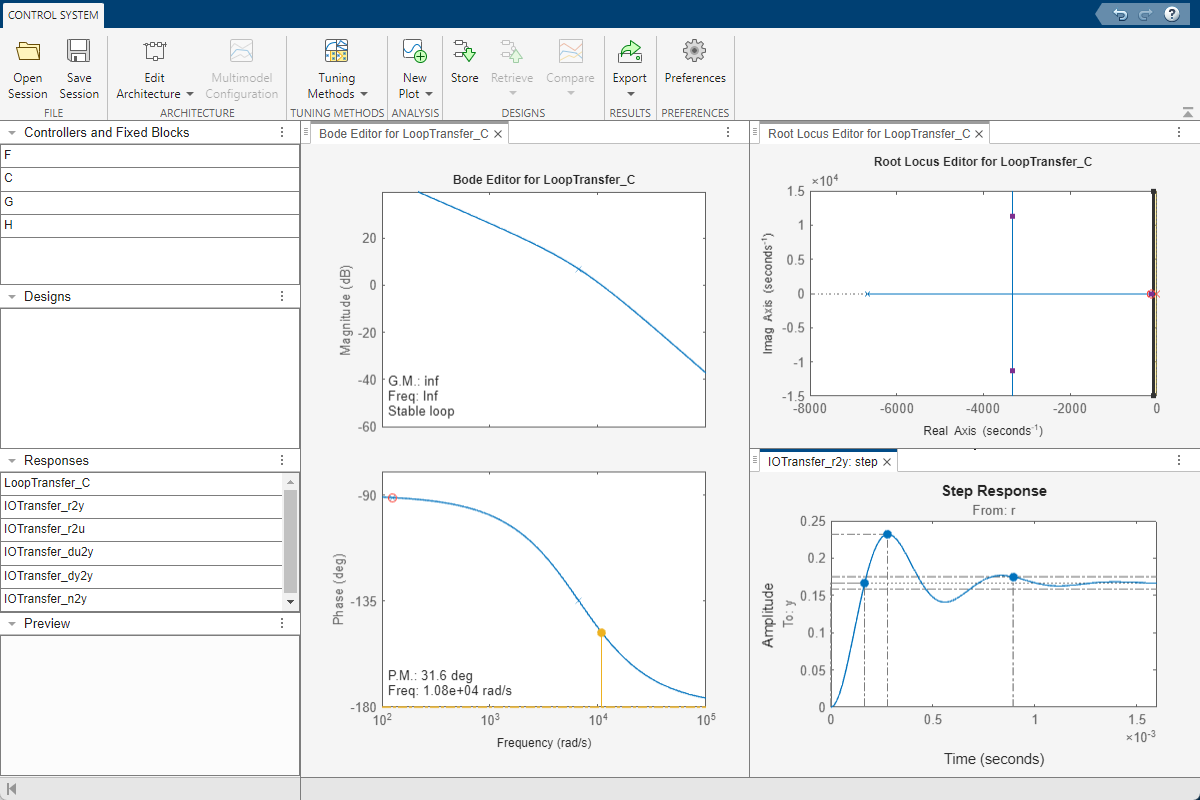
\includegraphics[scale=0.5]{FIG_M_gain6.png}
                    \end{center}
\end{figure}
\newpage
GAIN k = 1000 :
\begin{figure}[H]
        \begin{center}
                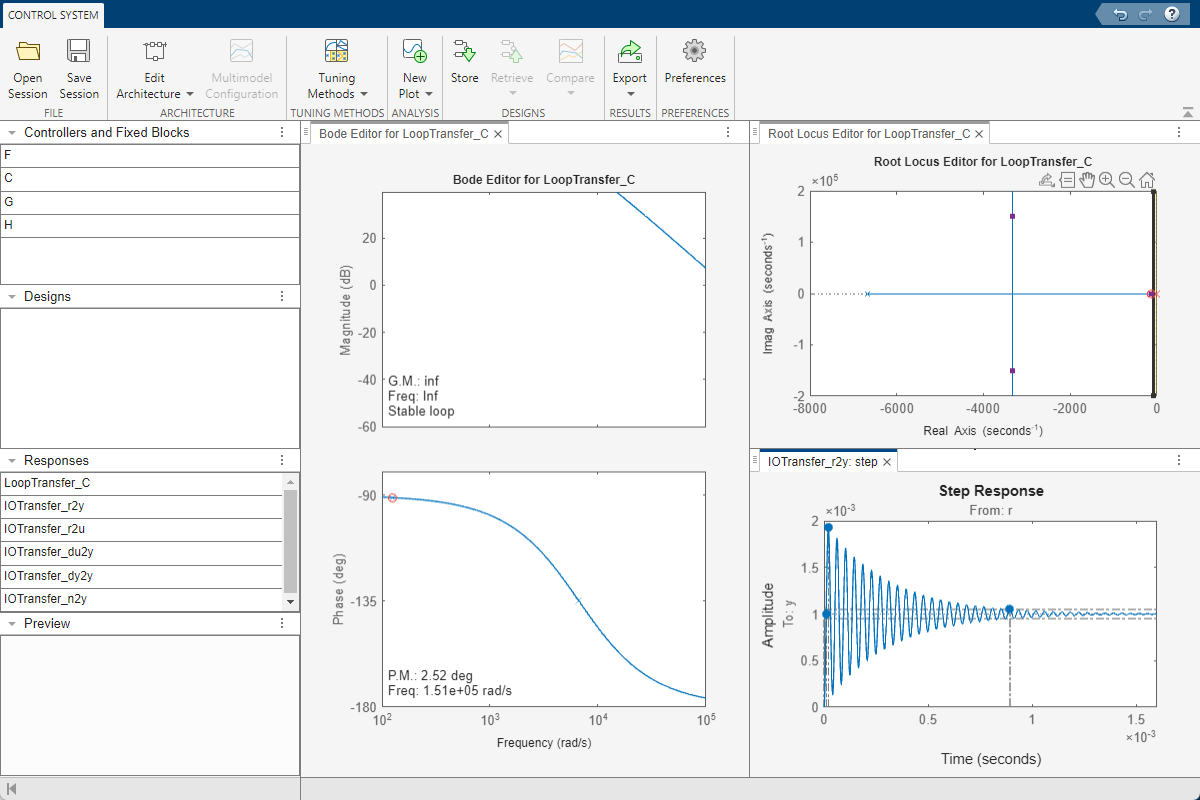
\includegraphics[scale=0.5]{FIG_M_gain1000.png}
                    \end{center}
\end{figure}



\newpage


%%%%%%%%%%%%%%%%%%%%%%%%%%%%%%%%%%%%
%       Conclusion 
%%%%%%%%%%%%%%%%%%%%%%%%%%%%%%%%%%%%
\section{Conclusion}
Ce laboratoire a permis d’analyser le comportement d’un banc de test SIRAu en reliant les mesures empiriques à une modélisation par fonction de transfert. Après avoir estimé la fonction de transfert du système, un régulateur PI a été appliqué pour obtenir une réponse en boucle fermée stable et performante.
\\\\Les diagrammes de Bode, Nyquist et Evans ont confirmé la stabilité du système, avec des marges de phase et de gain positives. Les réponses indicielles ont validé le réglage du régulateur, montrant un dépassement contrôlé et un temps de réponse adapté.
\\\\L’utilisation de MATLAB et de Control System Designer a permis de valider les résultats et de comparer les approches théoriques et pratiques. Ce travail a renforcé la compréhension des méthodes d’analyse des systèmes asservis et de leur application concrète

\newpage
\section{annexes (code inexact à cause du compilateur latex)}
\subsection{Code complet matlab exercice 2}
load('Z:\ MT\ systeme\_asservis\ SIRAu\_stepResponse.mat')
\\
\\t = time;
\\\\
\%\% Affichage propre des fonctions de transfert
    clear; close all; clc;
\\
s = tf('s');
\\
\\\%\% G moteur
\\K\_mot = 4.53e3;
\\tau\_mot = 8e-3;
\\G\_mot = K\_mot / (1 + tau\_mot*s);
\\
\\\%\% G element
\\K\_ele = 20.8e-3;
\\tau\_ele = 1.5e-4;
\\G\_ele = K\_ele / (1 + tau\_ele*s);
\\
\\\%\% G mesure
\\K\_mes = 10.7e-3;
\\G\_mes = tf(K\_mes);
\\
\\\%\% G systeme complet
\\G\_s = G\_mot * G\_ele * G\_mes;
\\
\\disp('===== G\_s =====')
\\G\_s
\\
\\\%\% D) Regulateur PI
\\k\_R = 3306;
\\T\_n = 8e-3;
\\
\\G\_R = k\_R * (1 + s*T\_n) / s;
\\
\\disp('===== G\_R =====')
\\G\_R
\\
\\\%\% Boucle ouverte
\\G\_0 = G\_R * G\_s;
\\
\\disp('===== G\_0 avant simplification =====')
\\G\_0
\\
\\\%\% Simplification
\\G\_0\_simpl = minreal(G\_0);
\\
\\disp('===== G\_0 apres simplification =====')
\\G\_0\_simpl
\\
\\\%\% Boucle fermee
\\G\_cf = feedback(G\_0\_simpl,1);
\\
\\disp('===== G\_cf =====')
\\G\_cf
\\
\\\%\% Recuperer numerateur et denominateur
\\[num,den] = tfdata(G\_cf,'v');
\\
\\disp('===== Numerateur de G\_cf =====')
\\num
\\
\\disp('===== Denominateur de G\_cf =====')
\\den
\\
\\\%\% Affichage de la forme Kcf / (a s\\$^$2 + b s + c)
\\K\_cf = num(end);
\\a = den(1);
\\b = den(2);
\\c = den(3);
\\
\\fprintf('\\nG\_cf(s) = \%.6f / (\%.6e s\\$^$2 + \%.6e s + \%.6e )\\n',K\_cf,a,b,c);
\\
\\\%\% Verification graphique
\\figure;
\\step(G\_cf);
\\grid on;
\\title('Reponse indicielle de G\_{cf}')
\\
\\\%\% Parametres temporels
\\info = stepinfo(G\_cf,'SettlingTimeThreshold',0.05,'RiseTimeLimits',[0 1]);
\\
\\Overshoot = info.Overshoot
\\RiseTime = info.RiseTime
\\SettlingTime = info.SettlingTime
\\
\\\%\% Bode et Nyquist de la boucle ouverte --> point E)
\\figure;
\\margin(G\_0\_simpl);
\\grid on;
\\title('Diagramme de Bode de G\_0')
\\
\\figure;
\\nyquist(G\_0\_simpl);
\\grid on;
\\
\\title('Diagramme de Nyquist de G\_0')
\\
\\
\\\%\% EVANS --> Point F
\\figure;
\\rlocus(G\_0\_simpl); \% trouver les yeros
\\grid on;
\\
\\figure;
\\step(G\_cf);

\subsection{Code python point I}
\\import numpy as np
\\import matplotlib.pyplot as plt
\\import control as ctrl
\\
\\# Fonction de transfert du système complet (à adapter)
\\s = ctrl.TransferFunction.s
\\G\_s = 1.008 / (1.2e-6 * s**2 + 0.00815 * s + 1)
\\
\\# Calcul des marges de stabilité
\\gm, pm, wg, wp = ctrl.margin(G\_s)
\\
\\# Tracé du diagramme de Bode avec légende détaillée
\\plt.figure(figsize=(10, 6))
\\plt.subplot(2, 1, 1)
\\ctrl.bode(G\_s, dB=True, Hz=False, omega=np.logspace(-1, 3, 1000), margins=True)
\\plt.title("Diagramme de Bode - Marges de stabilité")
\\plt.legend(
\\    [
\\        "Gain (dB)",
\\        "Phase (deg)",
\\        f"Marge de phase: {pm:.1f}°",
\\        f"Marge de gain: {gm:.1f} dB"
\\    ],
\\    loc='upper right'
\\)
\\
\\plt.tight\_layout()
\\plt.savefig("\_\_i2.png")
\\
\\# Affichage des valeurs
\\print(f"Marge de phase : {pm:.1f}°")
\\print(f"Marge de gain : {gm:.1f} dB")
\\
\\\subsection{Code python point K}
\\# Fonction de transfert en boucle fermée (à adapter)
\\G\_cf = ctrl.TransferFunction([1.008], [1.2e-6, 0.00815, 1])
\\
\\# Réponse indicielle
\\t, y = ctrl.step\_response(G\_cf)
\\
\\# Calcul des caractéristiques
\\overshoot = np.max(y) - 1  # Dépassement en %
\\settling\_time = np.where(np.abs(y - 1) < 0.05)[0][-1] * (t[1] - t[0])  # Temps d'établissement à 5%
\\rise\_time = np.where(y >= 1)[0][0] * (t[1] - t[0])  # Temps de montée (0 à 100%)
\\
\\# Tracé de la réponse indicielle avec légende détaillée
\\plt.figure(figsize=(10, 5))
\\plt.plot(t, y, label=f'Réponse indicielle\\nDépassement: {overshoot*100:.1f}%\nTemps de montée: {rise_time:.3f} s\nTemps d\'établissement: {settling_time:.3f} s')
\\plt.axhline(1, color='red', linestyle='--', label='Valeur finale')
\\plt.axvline(settling\_time, color='green', linestyle=':', label=f'Temps d\\'établissement: {settling\_time:.3f} s')
\\plt.axvline(rise\_time, color='orange', linestyle=':', label=f'Temps de montée: {rise\_time:.3f} s')
\\plt.title("Réponse indicielle - Caractéristiques")
\\plt.xlabel("Temps [s]")
\\plt.ylabel("Amplitude")
\\plt.legend(loc='upper left')
\\plt.grid(True)
\\plt.savefig("\_\_k2.png")
\\
\\# Affichage des valeurs
\\print("Caractéristiques de la réponse indicielle :")
\\print(f"Dépassement maximal: {overshoot*100:.1f}\%")
\\print(f"Temps de montée: {rise\_time:.3f} s")
\\print(f"Temps d'établissement: {settling\_time:.3f} s")

\subsection{Code python point L}
\\# Fonction de transfert du système complet
\\s = ctrl.TransferFunction.s
\\G\_s = 1.008 / (1.2e-6 * s**2 + 0.00815 * s + 1)
\\
\\# Gains du régulateur à tester
\\gains = [2500, 3306, 4500, 6000]
\\overshoots = []
\\
\\plt.figure(figsize=(12, 6))
\\for k in gains:
\\    # Régulateur PI
\\    G\_R = ctrl.TransferFunction([k * 8e-3, k], [1, 0])
\\    # Fonction de transfert en boucle fermée
\\    G\_cf = ctrl.feedback(G\_R * G\_s, 1)
\\    # Réponse indicielle
\\    t, y = ctrl.step\_response(G\_cf)
\\    overshoot = np.max(y) - 1  # Dépassement en %
\\    overshoots.append(overshoot * 100)
\\    plt.plot(t, y, label=f"Gain k={k}, Dépassement={overshoot*100:.1f}%")
\\
\\plt.title("Réponses indicielles pour différents gains du régulateur")
\\plt.xlabel("Temps [s]")
\\plt.ylabel("Amplitude")
\\plt.legend(loc='upper right')
\\plt.grid(True)
\\plt.xlim(0, 0.005)
\\plt.savefig("\_\_l2.png")
\\
\\# Tableau des résultats
\\print("Tableau des gains et dépassements :")
\\print("| Dépassement souhaité | Gain du régulateur | Valeur de dépassement (%) |")
\\print("|----------------------|--------------------|-----------------------------|")
\\for i, k in enumerate(gains):
\\    print(f"| {'4.3\%' if i==0 else '5.0\%' if i==1 else '10\%' if i==2 else '16.3\%'} | {k} | {overshoots[i]:.1f}\% |")

\end{document}


